
\documentclass[10pt, reqno]{amsart}
\usepackage[utf8]{inputenc}
\usepackage[T2A]{fontenc}
\usepackage[english,russian]{babel}
\usepackage{amsmath}
\usepackage{amssymb}
\usepackage{amsfonts}
\usepackage{graphicx}
\usepackage[hidelinks,unicode]{hyperref}


\def\udcs{519.233} %Here the author places classificators of the paper according to Russian classification system
\def\mscs{62F03} %Here the author places  classificators according to the AMS classification list.
\setcounter{page}{1}

\newtheorem*{theorem*}{Теорема}
\newtheorem{repeated_theorem}{Теорема}
\newtheorem{numbered_theorem}{Утверждение}
\newtheorem{numbered_corollary}{Замечание}
\newtheorem{lemma}{Лемма}

\newcommand{\norm}[1]{\left\lVert#1\right\rVert}

\DeclareUnicodeCharacter{2212}{-}
\DeclareMathOperator*{\E}{\mathbb{E}}
\DeclareMathOperator*{\Pb}{\mathbb{P}}

\def\logo{{\bf\huge S\raisebox{0.2ex}{\hspace{0.55ex}\raisebox{0.05ex}e\hspace{-1.65ex}$\bigcirc$}MR}}

\makeatletter
\def\@settitle{
    \begin{center}%
    \baselineskip14\p@\relax
    \bfseries
    \large
    \@title
  \end{center}%
}
\makeatother

\usepackage{graphicx}
\makeatletter
\providecommand{\bigsqcap}{%
  \mathop{%
    \mathpalette\@updown\bigsqcup
  }%
}
\newcommand*{\@updown}[2]{%
  \rotatebox[origin=c]{180}{$\m@th#1#2$}%
}
\makeatother


\begin{titlepage}
\author{{А.В. Резлер, М.Г. Чебунин}}%

\address{Alexandr Vadimovich Rezler
\newline\hphantom{iii} Novosibirsk State University
\newline\hphantom{iii} 2, Pirogova str.}%

\email{rezlers123@gmail.com}%
\address{Mikhail Georgievich Chebunin
\newline\hphantom{iii} Karlsruhe Institute of Technology,
\newline\hphantom{iii} Institute of Stochastics,
\newline\hphantom{iii} Karlsruhe, 76131, Germany,
\newline\hphantom{iii} Novosibirsk State University, 
\newline\hphantom{iii} 2, Pirogova str.,
\newline\hphantom{iii} Novosibirsk, 630090, Russia.}%

\email{chebuninmikhail@gmail.com}%
\end{titlepage}
\begin{document}
\renewcommand{\refname}{References}
\renewcommand{\proofname}{Доказательство.}
\renewcommand{\figurename}{Fig.}
\thispagestyle{empty}
\section{Постановка задачи}
Определим процесс бернулиевского града, падающего на горячую поверхность (Bernoulli Hail on a Hot Ground). Пусть время дискретно, и поверхность представляет из себя целочисленную прямую $\mathbb{Z}$. Предположим, что в каждый момент времени $n \in \mathbb{Z}_{+}$ в каждую точку $i \in \mathbb{Z}$ поверхности, с вероятностью $p$, незавсисмо от других параметров системы, приходит клиент, обозначаемый $\{i, i+1\}$ (клиент типа $i$) и ждет обслуживания. Каждому клиенту необходимо $h$ единиц времени $(h=1)$, чтобы завершить его. Обслуживание клиентов происходит в порядке FIFO (first in first out). Однако, в один момент времени, не может происходить обслуживание клиентов, стоящих рядом. В случае, если в один момент времени в систему пришли клиенты типа $i$ и $i+1$, то их порядок определяется случайным образом, а именно с вероятностью $1/2$ кто-то из них окажется первее. Построим граф $G(p)$, определяющий порядок обслуживания клиентов. Сперва рассмотрим случай $p=1$ и затем, на его основе, опишем граф для произвольного значения $p$. Узлами данного графа являются элементы множества $\{(i,n) : i \in \mathbb{Z} \text{,  } n \in \mathbb{Z}_{+}\}$. Ребро вида $(i_{1},n_{1}) \xrightarrow{} (i_{2},n_{2})$ означает, что клиент типа $i_{1}$, пришедший в момент времени $n_{1}$, не начнет обслуживание, пока клиент типа $i_{2}$, пришедший в момент времени $n_{2}$, не завершит его. Таким образом, учитывая ограничения модели, в каждой точке $(i, n)$, будем строить граф следующим образом:
\begin{enumerate} 
  \item[1.] Строим ребро $(i+1,n) \xrightarrow{} (i,n)$ с вероятностью $1/2$, либо ребро $(i,n) \xrightarrow{} (i+1,n)$ иначе.
  \item[2.] Строим ребра $(i,n) \xrightarrow{} (i-1,n-1)$, $(i,n) \xrightarrow{} (i,n-1)$, $(i,n) \xrightarrow{} (i+1,n-1)$ для всех $n \geq 2$.
\end{enumerate}
Теперь опишем граф $G(p)$, при $0 \leq p < 1$.
\begin{enumerate} 
  \item[1.] Закрасим каждый узел графа $G(1)$ с вероятностью $1-p$ в белый цвет и с вероятностью $p$ в черный
  \item[2.] Если узел $(i,n)$ белый, то удалим все смежные с ним ребра, кроме ребра $(i,n) \xrightarrow{} (i,n-1)$.
\end{enumerate}
Заметим, что, для данного графа справедливо \textbf{свойство монотонности}, то есть, при $p \leq q$, верно включение $G(p) \subseteq G(q)$.\\

Пусть $(i_{1},n_{1})$, $(i_{2},n_{2})$,..., $(i_{m},n_{m})$ --- последовательно соединенные узлы графа $G(p)$ (все ребра направлены вправо). Назовем данную последовательность \textbf{путем} длины $m$, начинающийся в узле $(i_{1},n_{1})$. Определим \textbf{высоту} пути как суммарное время обслуживания вдоль данного пути. Пусть теперь $H^{i}_{n} = H^{i}_{n}(p)$ --- максимальная высота среди всех путей, начинающихся в узле $(i,n)$ в графе $G(p)$. Покажем, что $H^{i}_{n}(p)$ ограничена. Учитывая свойство монотонности модели, а также однородность по пространству, достаточно это показать для $H^{0}_{n}(1)$. Пусть
\begin{equation*}
    t^{+}_{n,n} = \min\{i \geq 1: (i,n) \xrightarrow{} (i-1,n)\},
\end{equation*}
и для $m = n-1, n-2,..., 1$ определим
\begin{equation*}
    t^{+}_{m,n} = \min\{i > t^{+}_{m+1,n} + 1: (i,n) \xrightarrow{} (i-1,n)\}.
\end{equation*}
Аналогично, пусть
\begin{equation*}
    t^{-}_{n,n} = \max\{i \leq -1: (i,n) \xrightarrow{} (i+1,n)\},
\end{equation*}
и для $m = n-1, n-2,..., 1$
\begin{equation*}
    t^{-}_{m,n} = \max\{i < t^{-}_{m,n} - 1: (i,n) \xrightarrow{} (i+1,n)\}.
\end{equation*}
Тогда получим следующую оценку
\begin{equation}
    H^{0}_{n} \leq \sum_{i=1}^{n}(t^{+}_{i,n} - t^{-}_{i,n}) + n
    \label{Height_rough_est}
\end{equation}
Теперь, с помощью полученной оценки, оценим математическое ожидание $H^{i}_{n}$. Сперва найдем распределения случайных величин $\{t^{+}_{m,n}\}$, при $n \geq 1$ и $1 \leq m \leq n$ (для $\{t^{-}_{m,n}\}$ рассуждение аналогично). Сперва заметим, что
\begin{equation*}
    t^{+}_{m,n} - (t^{+}_{m+1,n} + 1) \overset{d}{=} t^{+}_{m,m}.
\end{equation*}
Тогда ясно, что
\begin{equation*}
    t^{+}_{m,n} \overset{d}{=} \sum_{k=0}^{m-n}t^{+}_{m+k,m+k} + (n-m).
\end{equation*}
Найдем распределение $t^{+}_{m,m}$. Так как
\begin{equation*}
    \{t^{+}_{m,m} = k\} = \{(0,m) \xrightarrow{} (1,m), (1,m) \xrightarrow{} (2,m),..., (k-2,m) \xrightarrow{} (k-1,m), (k-1,m) \xleftarrow{} (k, m)\},
\end{equation*}
где $k \geq 1$, получим следующее распределение случайной величины $t^{+}_{m,m}$
\begin{equation*}
    \Pb(t^{+}_{m,m} = k) = 2^{-k}.
\end{equation*}
Тогда, для математического ожидания случайной величины $t^{+}_{m,m}$ получим
\begin{equation}
    \E{}t^{+}_{m,m} = \sum_{k=1}^{\infty}\Pb(t^{+}_{m,m} \geq k) = \sum_{k=1}^{\infty}2^{-k+1} = \sum_{k=0}^{\infty}2^{-k} = 2
    \label{me_t+}
\end{equation}
Итого, учитывая формулы (\ref{Height_rough_est}) и (\ref{me_t+}), для математического ожидания $H^{0}_{n}$ получим
\begin{equation}
    \E{}H^{0}_{n} \leq \sum_{i=1}^{n}6(n-i+1) + n = O(n^{2})
\end{equation}

\section{Вопросы}
\begin{enumerate} 
  \item[1.] Оценка производных для приближения по формуле Тейлора?
  \item[2.] Возможно ли построить каплинг для данной модели со свойствами суб/супер аддитивности?
  \item[3.] Можно ли получить оценки для предельных констант в случае, если вместо исходной поверхности будем рассматривать окружность с тремя точками? С произвольным количеством точек?
  \item[4.] Можно ли комбинаторными методами найти распределение $H_{n}^{i}$, при некоторых допущениях для модели?
  \item[5.] Провести компьютерную симуляцию модели.
\end{enumerate}
\newpage
  3.1. Рассмотрим сперва случай $p=1$. В силу правил построения ребер на одном временном уровне $(t - Fix)$, а также определения величины $H_{n}^{i}(p)$ ясно, что максимальная длина очереди на каждом временном уровне равна $3$, а также, так как от каждого черного узла будет выходить три ребра на нижестоящий уровень, то ни один клиент, пришедший в момент времени $n$ не будет обслужен, пока не закончат обслуживания клиенты на уровне $n-1$. Таким образом, легко выписать распределение для $H_{n}^{i}(1)$, где $i=1,2,3$ и $n \geq 0$.
  
  \begin{equation}
      H_{n}^{i} = \begin{cases}
      3n-2, & \text{prob} = 1/3 \\
      3n-1, & \text{prob} = 1/3 \\
      3n, & \text{prob} = 1/3 \\
      \end{cases}
  \end{equation}

  Пусть теперь $0 < p < 1$. Аналогично предыдущему случаю, можно заметить, что клиенты, пришедшие в момент времени $n$ не будут обслужены, пока не завершится обслуживание клиентов, пришедших на уровень $n-1$. Таким образом, искомую случайную величину $H_{n}^{i}$ можно выразить в виде суммы двух независимых случайных величин $\xi_{n}^{i}$ -- длина очереди на уровне $n$ и $B(3n-3, p)$ -- биномиальная случайная величина с параметрами $3n-3$ и $p$. Итого получим
  
  \begin{equation}
      H_{n}^{i} = \xi_{n}^{i} + B(3n-3, p)
      \label{decomposition_of_H_for_3_case}
  \end{equation}
  
  Распределение $\xi_{n}^{i}$ легко находится обычным перебором, поэтому приведем только результат вычислений
  
  \begin{equation}
      \xi_{n}^{i} = \begin{cases}
      0, & \text{prob} = 1-p \\
      1, & \text{prob} = p - p^{2} + \frac{1}{4}p^{3} \\
      2, & \text{prob} = p^{2}(1-p/2) \\
      3, & \text{prob} = \frac{1}{4}p^{3}
      \end{cases}
  \end{equation}
  
  Распределение $H_{n}^{i}$ несложно найти, например, по формуле полной вероятности. Коэффициент линейного роста можно найти из формулы \ref{decomposition_of_H_for_3_case}, с помощью закона больших чисел. Итого получим
  
  \begin{equation}
      H_{n}^{i}/n \xrightarrow{} 3p \:\:\:\: i = 1,2,3.
  \end{equation}
  
  4.1 Найдем оценку для распределения $H_{n}^{0}$ "напрямую". Для этого воспользуемся следующими рассуждениями
  
  \begin{align*}
    \Pb(H_{n}^{0} = k) = \Pb(\exists \text{ путь длины } k \text{ и } \neg\exists \text{ пути длины } k+1) \\ = 1 - \Pb(\neg\exists \text{ пути длины } k \text{ или } \exists \text{ путь длины } k+1) \\ \geq 1 - \Pb(\neg\exists \text{ пути длины } k) - \Pb(\exists \text{ путь длины } k+1) \\ = \Pb(\exists \text{ путь длины } k) - \Pb(\exists \text{ путь длины } k+1)
  \end{align*}
  
  Теперь найдем вероятность событий $\{\exists \text{ путь длины } k\}$ для всех $k \geq 0$. Сперва заметим, что если мы зафиксируем точку откуда путь будет "стартовать" (пусть $(0,m)$), а также длину пути $k$, то количество различных конфигураций пути с заданными параметрами зависит от количества вариантов разложения числа $k$ в сумму из $m$ слагаемых $n_{1}, n_{2},...,n_{m}$, где $n_{i}$ можно интерпретировать как длину части исходного пути на $i$-ом временном уровне, и количества вариантов разложить заданную конфигурацию частей пути. Обозначим далее через $l_{i}$ -- части исходного пути, то есть $l_{1}+l_{2}+...+l_{m} = H_{m}^{0}$. Найдем вероятность события $\{l_{1}=n_{1}, l_{2}=n_{2},..., l_{m}=n_{m}\}$
  
  \begin{align*}
    \Pb(l_{1}=n_{1}, l_{2}=n_{2},..., l_{m}=n_{m}) \\ = p2^{I(n_{m}>1)}\Pb(l_{m}=n_{m})\cdot3^{I(n_{m-1}>0)}2^{I(n_{m-1}>1)}\Pb(l_{m-1}=n_{m-1})\cdot...\\ \cdot3^{I(n_{1}>0)}2^{I(n_{1}>1)}\Pb(l_{1}=n_{1}).
  \end{align*}
  
  Заметим, что $l_{1}, l_{2},..., l_{m}$ -- независимые одинаково распределенные случайные величины. Найдем распределение $l_{1}$
  
  \begin{align*}
    \Pb(l_{1} = n_{1}) = p^{n_{1}}(\frac{1}{2})^{n_{1}-1}((1-p)^{2} + 2\frac{1}{2}(1-p) + (\frac{1}{2})^{2}) = \frac{1}{2}(\frac{p}{2})^{n_{1}}(3-2p)
  \end{align*}
  
  Таким образом, получим
  
  \begin{align}
    \Pb(l_{1}=n_{1}, l_{2}=n_{2},..., l_{m}=n_{m}) \notag\\ = p3^{\sum_{i=1}^{m}I(n_{i}>0)}2^{\sum_{i=1}^{m}I(n_{i}>1)}2^{m}(\frac{p}{2})^{\sum_{i=1}^{m}n_{i}}(1-\frac{p}{2})^{2\sum_{i=1}^{m}I(n_{i}>0)}(1-p)^{\sum_{i=1}^{m}I(n_{i}=0)}
    \label{time_level_path_prob}
  \end{align}
  
  Для события $\{\exists \text{ путь длины } k\}$ имеем
  
  \begin{align*}
    \Pb(\exists \text{ путь длины } k) = \sum_{n_{1}+n_{2}+...+n_{m} = k}\Pb(l_{1}=n_{1}, l_{2}=n_{2},..., l_{m}=n_{m})
  \end{align*}
  
  Разобъем множество $A = \{n_{1}, n_{2},..., n_{m} \: : \: n_{1}+n_{2}+...n_{m}=k\}$ на такие подмножества, что на каждом из них индикаторные функции в выражении (\ref{time_level_path_prob}) принимают фиксированные значения. Обозначим через $Z_{i}^{m} = \{n_{1}, n_{2},..., n_{m} \: : \: i \text{ слагаемых равны нулю и } n_{1}+n_{2}+...n_{m}=k\} = \{n_{1}, n_{2},..., n_{m-i} \:\: : \:\: n_{1}+n_{2}+...+n_{m-i}=k\}$, а также $O_{i}^{m} = \{n_{1}, n_{2},..., n_{m} \: : \: j \text{ слагаемых равны } 1 \text{ и } n_{1}+n_{2}+...+n_{m}=k\} = \{n_{1}, n_{2},..., n_{m-i} \: : \: n_{1}+n_{2}+...+n_{m-i}=m-i\}$. Тогда, при условии, что значение $k$ и $m$ достаточно велики и $k > m$, для события $A$ имеем следующее разложение
  
  \begin{align*}
    A = \bigsqcup_{i=0}^{m-1}\bigsqcup_{j=0}^{m-i-1}A \cap Z_{i}^{m} \cap O_{j}^{m-i-1}
  \end{align*}
  
  Найдем мощность каждого подмножества в разложении. Для этого сперва заметим, что задача нахождения мощности множества $A \cap Z_{i}^{m} \cap O_{j}^{m-i-1}$ для некоторых $i, j$ сводится к комбинаторной задаче о количестве вариантов распределить $k-2(m-1-i-j)-j$ шаров по $m-1-i-j$ ящикам. Таким образом получаем
  
  \begin{align*}
    |A \cap Z_{i}^{m} \cap O_{j}^{m-i-1}| = C_{m-1}^{i}C_{m-1-i}^{j}C_{k-2(m-1-i-j)-j+m-1-i-j-1}^{m-1-i-j-1} \\ = C_{m-1}^{i}C_{m-1-i}^{j}C_{k-m+i}^{m-i-j-2}
  \end{align*}
  
  Теперь заметим, что на множестве $A \cap Z_{i}^{m} \cap O_{j}^{m-i-1}$ для некоторых $i, j$ имеем
  
  \begin{align*}
    \Pb(l_{1}=n_{1}, l_{2}=n_{2},..., l_{m}=n_{m}) \\ = p3^{m-i}2^{m-i-j}2^{m}(\frac{p}{2})^{k}(1-\frac{p}{2})^{2(m-i)}(1-p)^{i}
  \end{align*}
  
  Итого для события $\{\exists \text{ путь длины } k\}$ получим
  
  \begin{align*}
    \Pb(\exists \text{ путь длины } k) = \sum_{n_{1}+n_{2}+...+n_{m} = k}\Pb(l_{1}=n_{1}, l_{2}=n_{2},..., l_{m}=n_{m}) \\ = \sum_{i=0}^{m-1}\sum_{j=0}^{m-i-1}C_{m-1}^{i}C_{m-1-i}^{j}C_{k-m+i}^{m-i-j-2}p3^{m-i}2^{m-i-j}2^{m}(\frac{p}{2})^{k}(1-\frac{p}{2})^{2(m-i)}(1-p)^{i}
  \end{align*}
  
  4.2 Пусть теперь в системе всего $k+1$ сервер. Обозначим $h_{t}$ -- максимальная длина пути на временном уровне $t$. Тогда ясно, что справедлива следующая оценка
  
  \begin{equation}
      H_{n}^{i} \leq \sum_{t=1}^{n}h_{t} \:\:\:\: i=0,1,...,k.
  \end{equation}
  
  Легко понять, что $\{h_{t}\}_{t=0}^{\infty}$ -- независимые одинаково распределенные случайные величины. Таким образом, чтобы получить оценку сверху для искомого коэффициента линейного роста, с помощью закона больших чисел, достаточно найти математическое ожидание $h_{1}$. Для этого воспользуемся следующей формулой
  
  \begin{equation*}
      \E h_{1} = \sum_{j=0}^{k}\Pb(h_{1} \geq j).
  \end{equation*}
  
  Можно заметить, что 
  \begin{equation*}
      \Pb(h_{1} \geq j) = \Pb(\{\exists \text{ путь длины } j\}).
  \end{equation*}
  
  Найдем вероятность события $\{\exists \text{ путь длины } j\}$
  
  \begin{align*}
     \Pb(\{\exists \text{ путь длины } j\}) = 2(p/2)^{k+1} + 4(p/2)^{k}(1-p/2) + 6(p/2)^{k-1}(1-p/2)^{2} \\ + 8(p/2)^{k-2}(1-p/2)^{2} + ... + 2(k-j+2)(p/2)^{j}(1-p/2)^{2} \\ = 2(p/2)^{k+1} + 4(p/2)^{k}(1-p/2) + \sum_{i=2}^{k-j+1}2(i+1)(p/2)^{k-i+1}(1-p/2)^{2} \\ = 2(p/2)^{k+1} + 4(p/2)^{k}(1-p/2) + 2(p/2)^{k+1}(1-p/2)^{2}\sum_{i=2}^{k-j+1}(i+1)(p/2)^{-i}
  \end{align*}
  
  Посчитаем последнюю сумму отдельно
  
  \begin{align*}
     \sum_{i=2}^{k-j+1}(i+1)(p/2)^{-i} = (p/2)^{-1}\Big(\sum_{i=1}^{k-j}i(p/2)^{-i} + 2\sum_{i=1}^{k-j}(p/2)^{-i}\Big) \\ = (p/2)^{-1}\Big(\sum_{i=1}^{k-j}\sum_{s=i}^{k-j}(p/2)^{-s} + 2\sum_{i=1}^{k-j}(p/2)^{-i}\Big) \\ = (p/2)^{-1}\Big(\sum_{i=1}^{k-j}(p/2)^{-i}\frac{(1-(p/2)^{-(k-j+1-i)})}{(1-(p/2)^{-1})} + 2(p/2)^{-1}\frac{(1-(p/2)^{-(k-j)})}{(1-(p/2)^{-1})}\Big) \\ = \frac{(p/2)^{-1}}{(1-(p/2)^{-1})}\Big(\sum_{i=1}^{k-j}(p/2)^{-j} - \sum_{i=1}^{k-j}(p/2)^{-(k-j+1)} + 2(p/2)^{-1}(1-(p/2)^{-(k-j)})\Big) \\ = \frac{(p/2)^{-2}}{(1-(p/2)^{-1})}\Big(\frac{1-(p/2)^{-(k-j)}}{1-(p/2)^{-1}} - (k-j)(p/2)^{-(k-j)} + 2(1-(p/2)^{-(k-j)})\Big)
  \end{align*}
  
  Таким образом, итого для распределения имеем
  \begin{align*}
      \Pb(\{\exists \text{ путь длины } j\}) = 2(p/2)^{k+1} + 4(p/2)^{k}(1-p/2) + 2(p/2)^{k+1}(1-p/2)^{2}\frac{(p/2)^{-2}}{(1-(p/2)^{-1})}\\\cdot\Big(\frac{1-(p/2)^{-(k-j)}}{1-(p/2)^{-1}} - (k-j)(p/2)^{-(k-j)} + 2(1-(p/2)^{-(k-j)})\Big)
  \end{align*}
  
  5. Для компьютерной симуляции использовались языки программирования python и c++. Задача состояла в реализации алгоритма вычисления $H_{n}^{0}$. Однако в силу ограничения компьютерных мощностей, вместо инициализации множества узлов $\{(i, t) \: : \: i \in \mathbb{Z}, \: 0 \leq t \leq m\}$ для некоторого $m > 0$, производилась инициализация множества $\{(i, t) \: : \: i \in [-k, k], \: 0 \leq t \leq m\}$ для некоторого $k > 0$. В данной задаче Python используется для визуализации данных, однако его производительность сравнительно низкая, поэтому для вычисления алгоритма при больших значениях $k$ и $m$ используется c++, а python только вызывает скомпилированный код. Сперва рассмотрим графики средних значений на 100 реализациях функции $H_{n}^{0}(p)/n$ при фиксированном значении $n=10^{4}$ и значениях $p=0.05, 0.1, 0.2,..., 0.9$.\\\\
  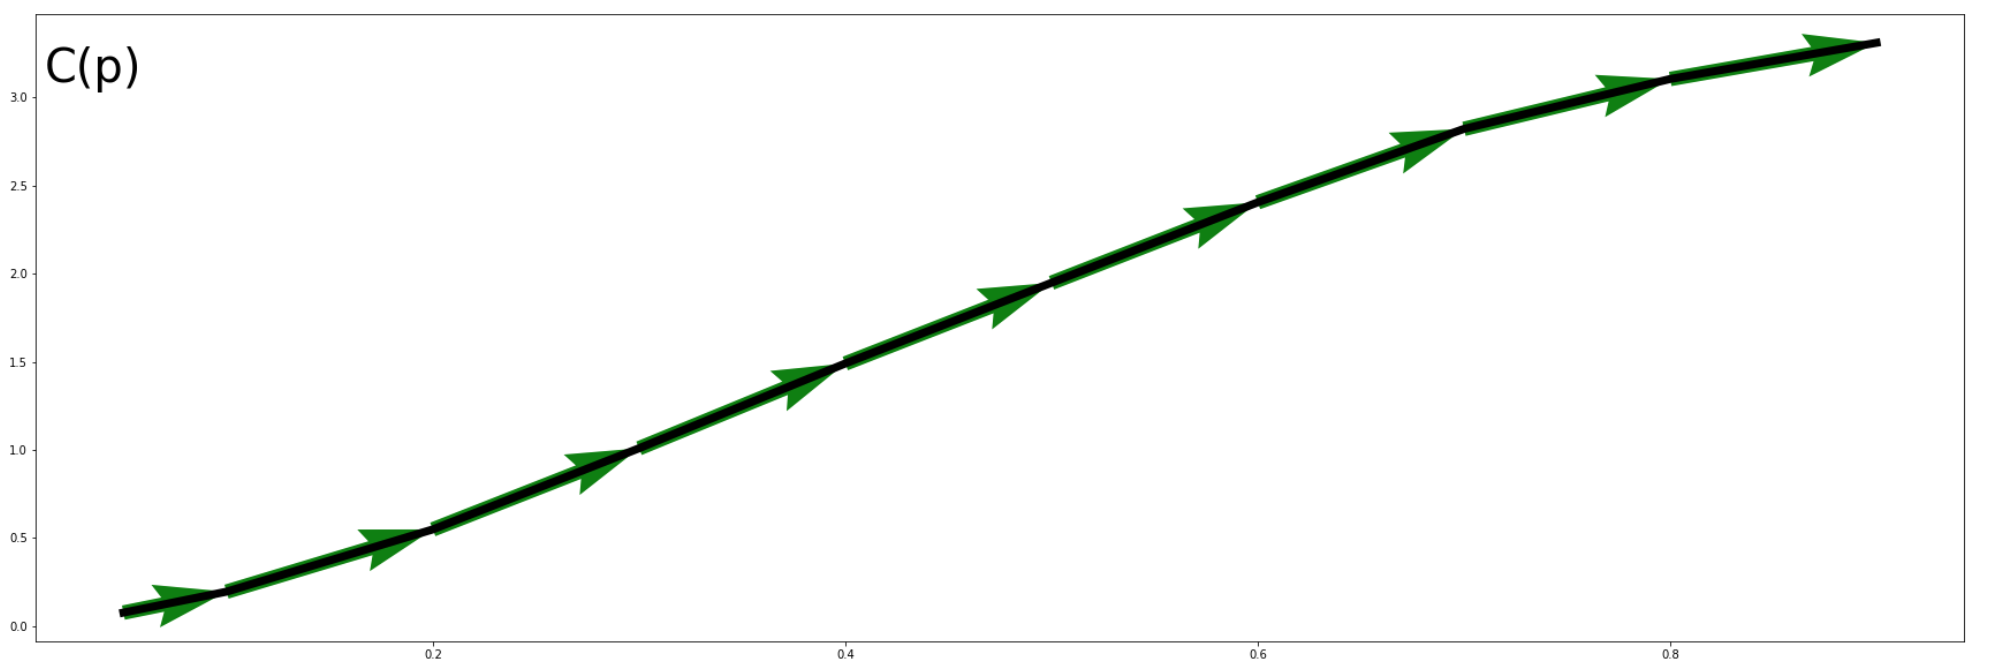
\includegraphics[width=10cm, height=5cm]{c(p).png}
  \\\\
  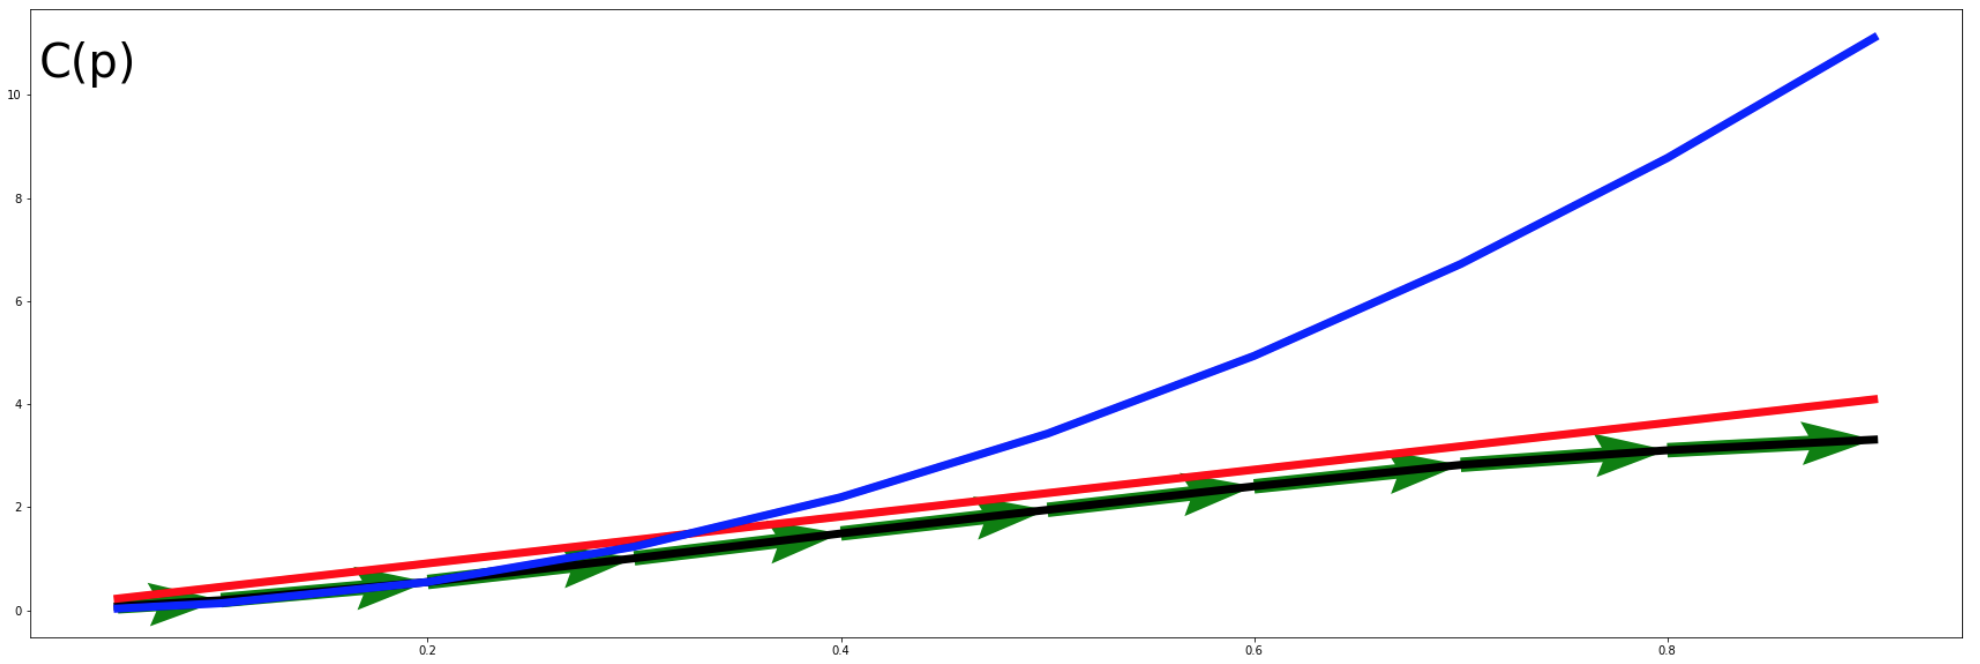
\includegraphics[width=10cm, height=5cm]{c(p)_lin_sq.png}
  \\\\
  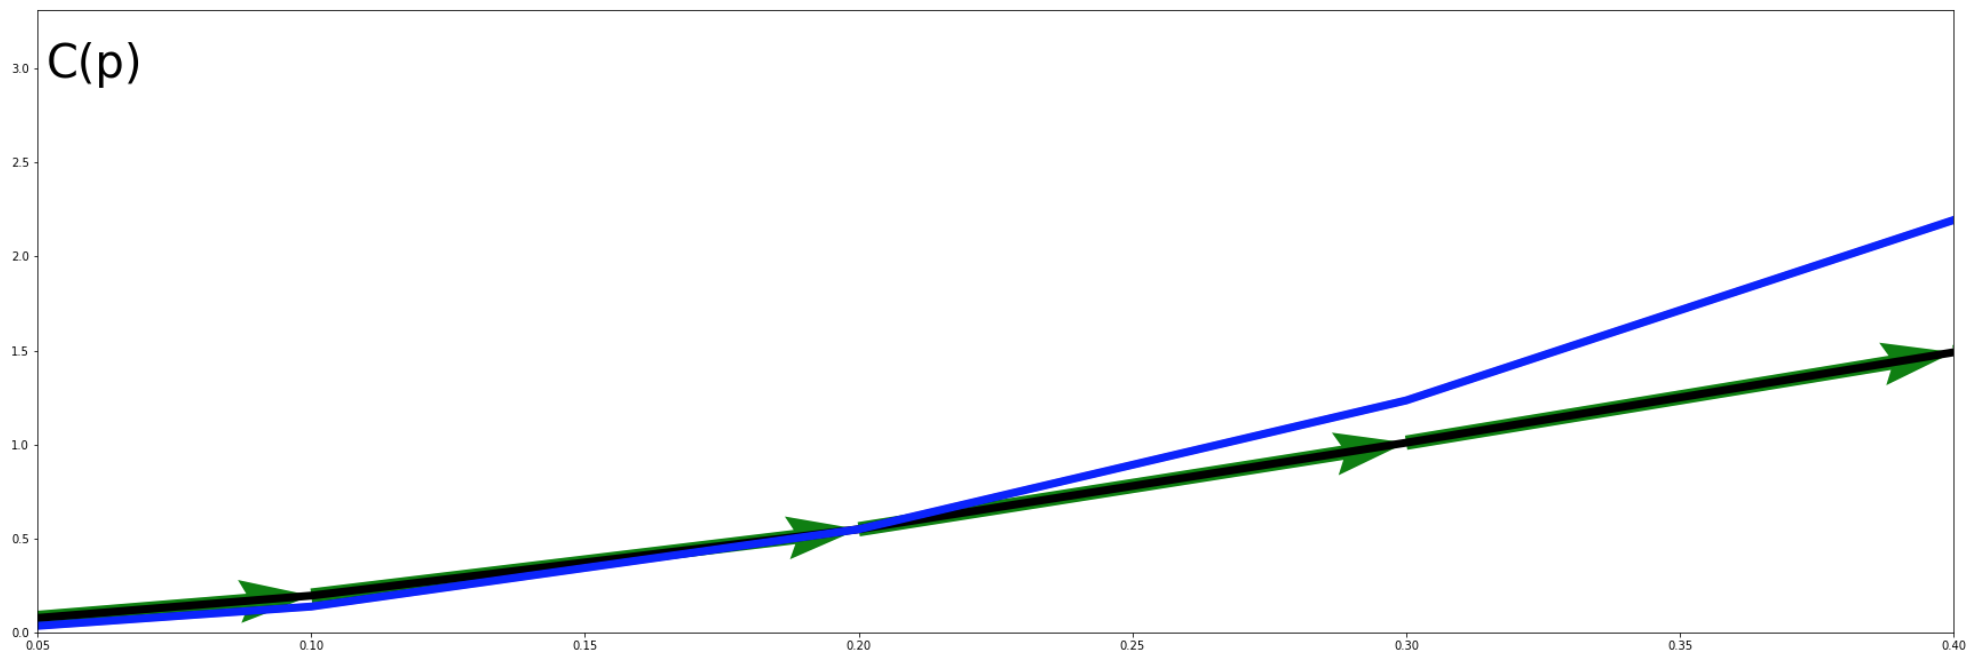
\includegraphics[width=10cm, height=5cm]{c(p)_sq_zoom.png}
  \\\\
  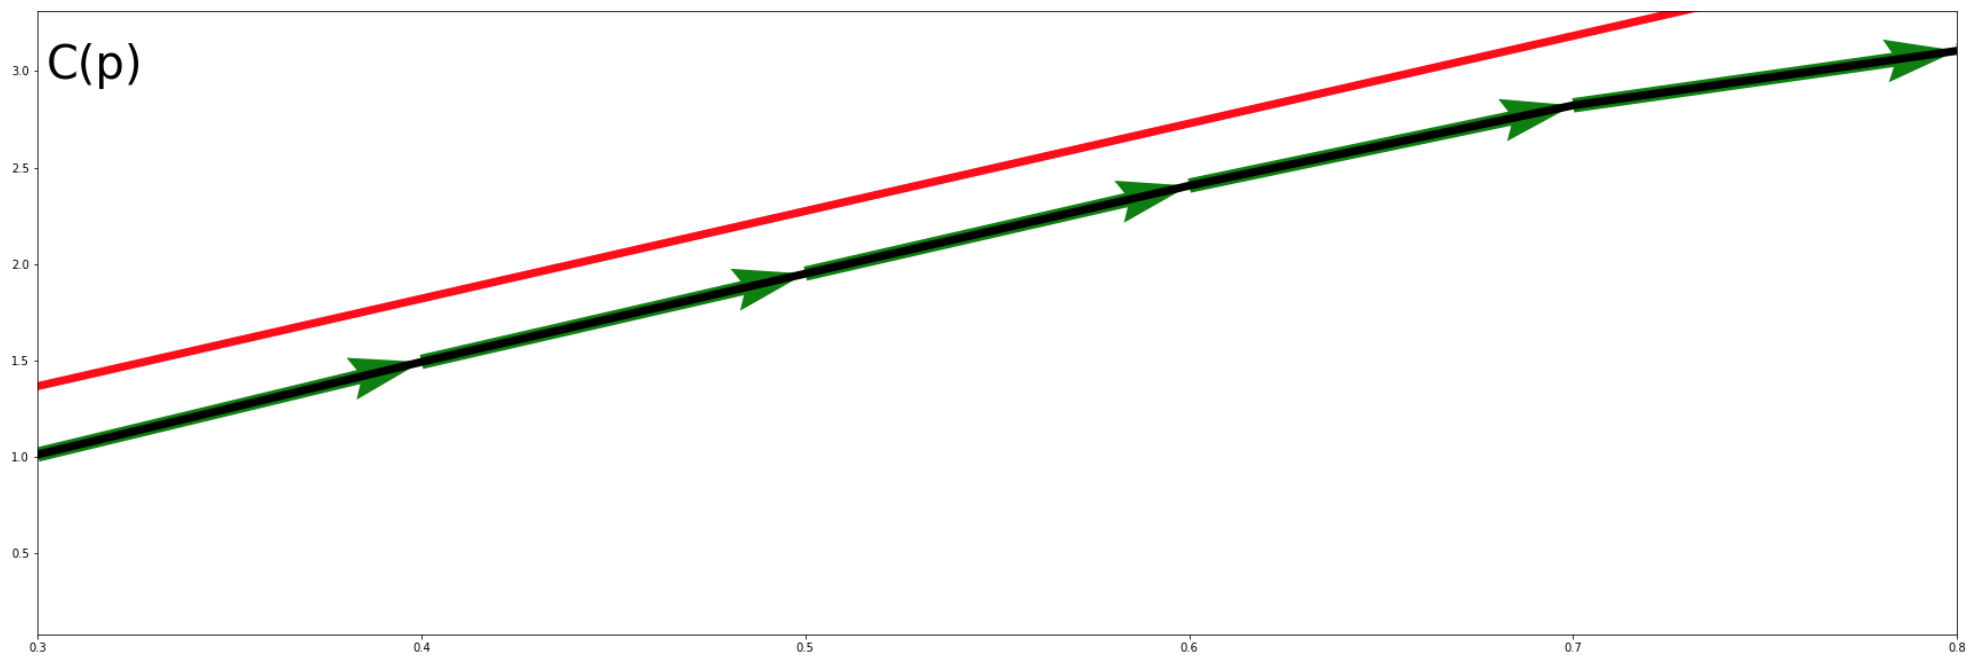
\includegraphics[width=10cm, height=5cm]{c(p)_lin_zoom.png}
  \\\\
  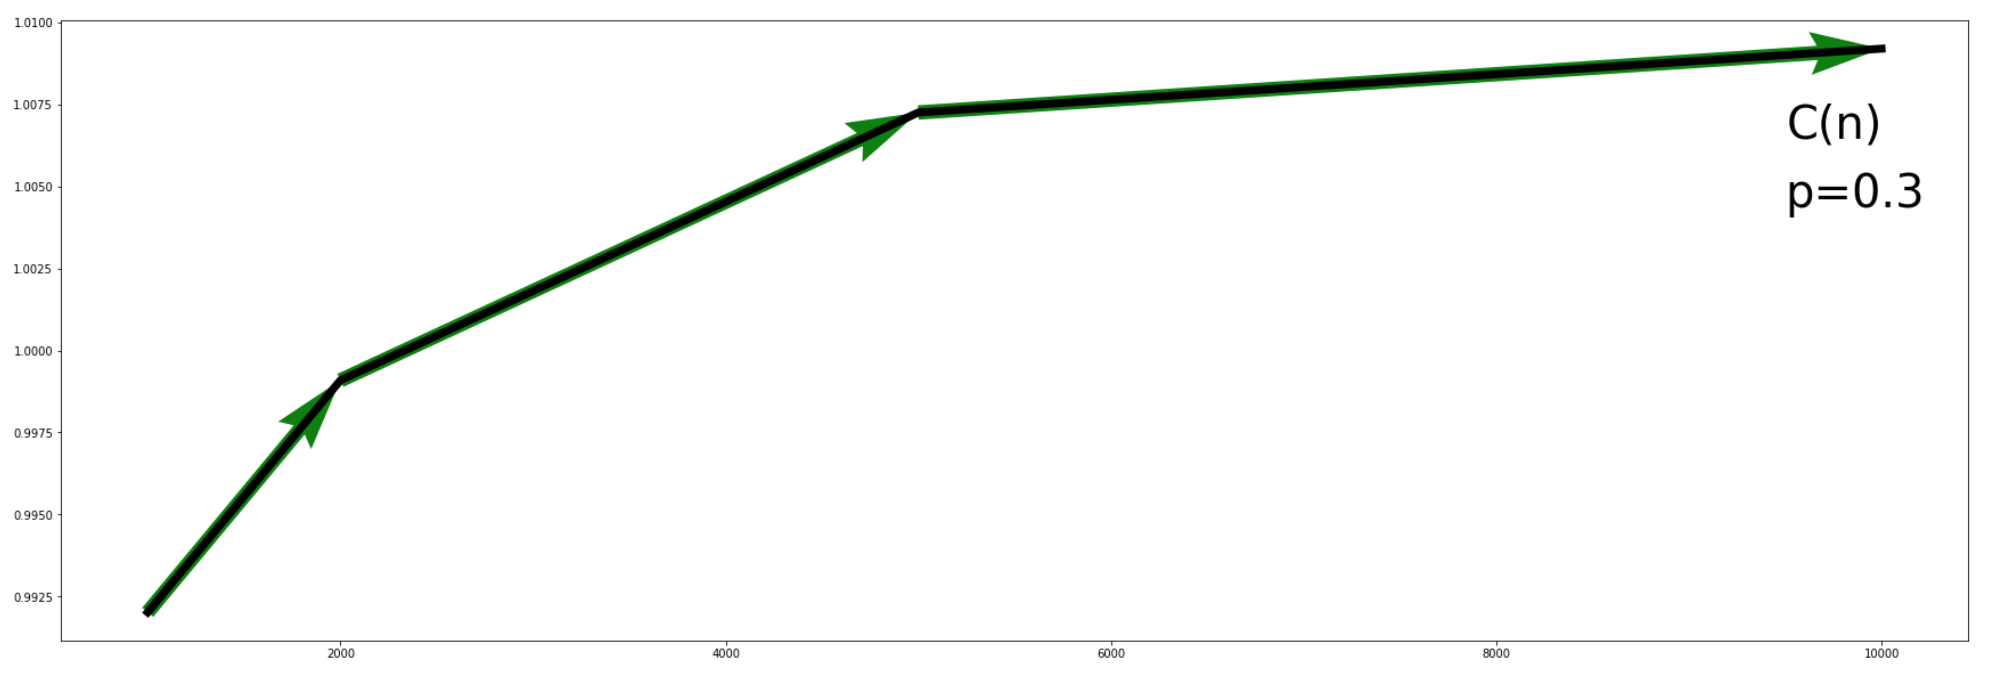
\includegraphics[width=10cm, height=5cm]{c(n)_03.png}
  \\\\
  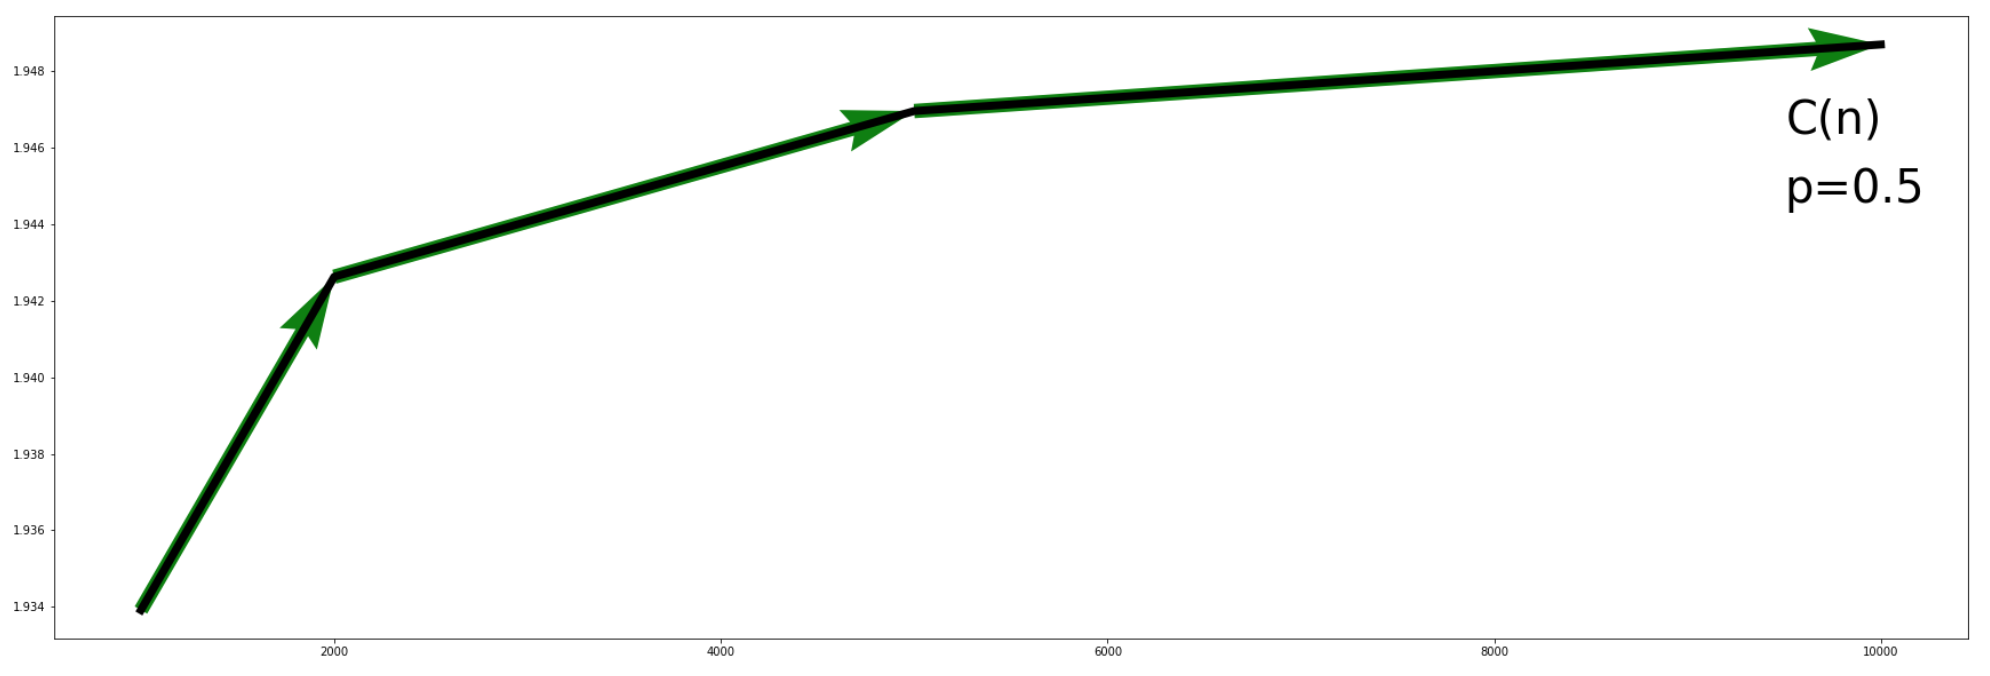
\includegraphics[width=10cm, height=5cm]{c(n)_05.png}
  \\\\
  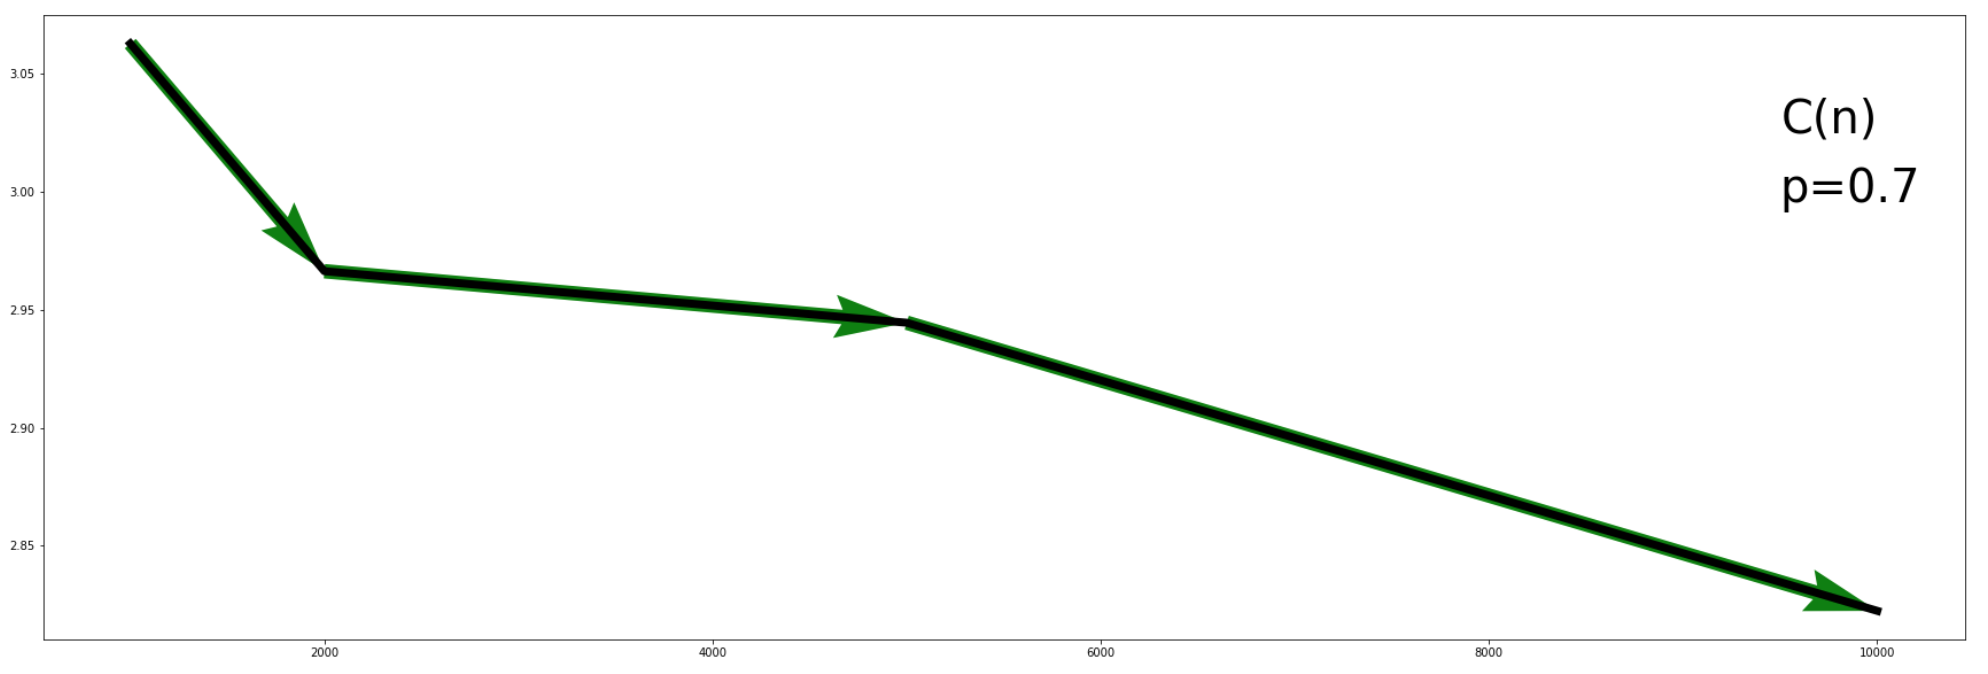
\includegraphics[width=10cm, height=5cm]{c(n)_07.png}
  \\\\
  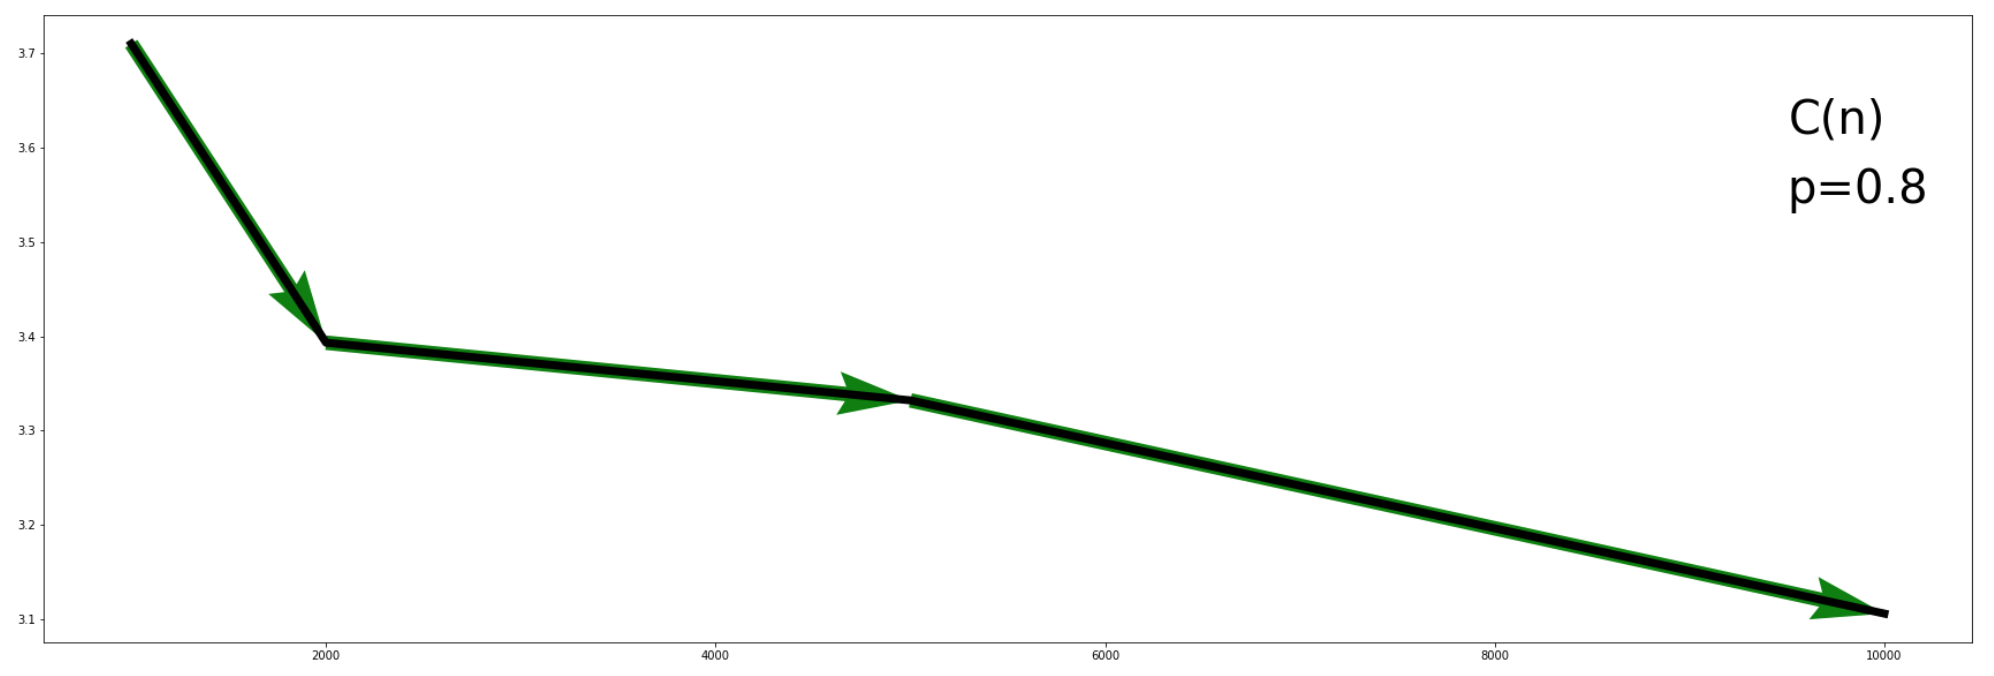
\includegraphics[width=10cm, height=5cm]{c(n)_08.png}
  \\\\
  \newpage
\end{document}



